\documentclass[a4paper,11pt]{article}
\usepackage{mathtools}
\usepackage[T1]{fontenc}
\usepackage[utf8]{inputenc}
\usepackage{graphicx}
\usepackage{xcolor}
\usepackage{verbatim}
\usepackage{amsmath}
\usepackage{array}
\usepackage{amssymb}
\usepackage{mathtools}
\usepackage{graphicx}
\usepackage{epstopdf}
\usepackage{inputenc}
\usepackage{breqn}
\usepackage{geometry}
\usepackage[linesnumbered,ruled]{algorithm2e}
\usepackage{amsmath}
\usepackage{amsmath,amssymb}
\usepackage{bm}
\usepackage{eqparbox}
\DeclareMathOperator{\E}{\mathbb{E}}
\usepackage{etoolbox}  % patch def of algorithmic environment
\makeatletter
\patchcmd{\algorithmic}{\addtolength{\ALC@tlm}{\leftmargin} }{\addtolength{\ALC@tlm}{\leftmargin}}{}{}
\makeatother
\usepackage[
pdftitle={Assignment 2}, 
pdfauthor={Yash Gangrade, University of Utah},
colorlinks=true,linkcolor=black,urlcolor=blue,citecolor=blue,bookmarks=true, bookmarksopenlevel=2]{hyperref}
\usepackage{amsmath,amssymb,amsthm,textcomp}
\usepackage{enumerate}
\usepackage{multicol}
\usepackage{tikz}
\usepackage{imakeidx}
\makeindex[columns=3, title=Alphabetical Index, intoc]
\usepackage{geometry}
\usepackage{algorithm, algorithmicx, algpseudocode}
\usepackage{mdframed}
\geometry{total={210mm,297mm},
left=20mm,right=20mm,%
bindingoffset=0mm, top=20mm,bottom=20mm}

\linespread{1.1}
\DeclareUnicodeCharacter{2212}{\in} 
\newcommand{\linia}{\rule{\linewidth}{0.5pt}}
\newcommand\Myperm[2][^n]{\prescript{#1\mkern-2.5mu}{}P_{#2}}
\newcommand\Mycomb[2][^n]{\prescript{#1\mkern-0.5mu}{}C_{#2}}
% custom theorems if needed
\newtheoremstyle{mytheor}
    {1ex}{1ex}{\normalfont}{0pt}{\scshape}{.}{1ex}
    {{\thmname{#1 }}{\thmnumber{#2}}{\thmnote{ (#3)}}}

\theoremstyle{mytheor}
\newtheorem{defi}{Definition}

\graphicspath{{Figures/}}

% my own titles
\makeatletter
\renewcommand{\maketitle}{
\begin{center}
\vspace{2ex}
{\huge \textsc{\@title}}
\vspace{1ex}
\\
\linia\\
\@author \hfill \@date
\vspace{4ex}
\end{center}
}
\makeatother
%%%

% custom footers and headers
\usepackage{fancyhdr,lastpage}
\pagestyle{fancy}
\lhead{}
\chead{}
\rhead{}
\lfoot{Assignment \textnumero{} 2}
\cfoot{}
\rfoot{Page \thepage\ of \ \pageref*{LastPage}}
\renewcommand{\headrulewidth}{0pt}
\renewcommand{\footrulewidth}{0pt}
%

%%%----------%%%----------%%%----------%%%----------%%%

\begin{document}

\title{CS 6635: Visualization of Scientific Data Homework 2 \\ \large ParaView}

\author{Yash Gangrade (u1143811), MS First Year, School of Computing}

\date{10\textsuperscript{th} February 2017}
\maketitle
\tableofcontents
\listoffigures
\null \clearpage

%%%%%%%%%%%%%%%%%%% Main Content %%%%%%%%%%%%%%%%%%%
%%%%%%%%%%%%%%%%%%% Part I %%%%%%%%%%%%%%%%%%%
%%%%%%% Question 1 %%%%%%%
\section{Part 1}
\subsection{Visualization of Statistics for 1-D Data}
\paragraph{Ans.}
The line charts and the histogram plot from the ParaView are attached below. The related questions are also answered below the diagrams.

\begin{figure}[!h]
    \centering
    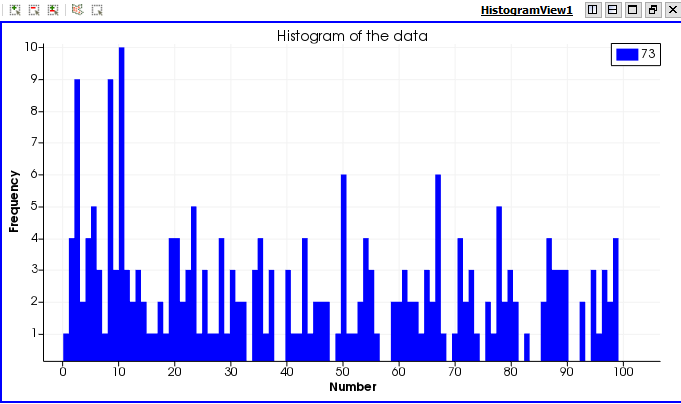
\includegraphics[scale=0.95]{Q1_H.PNG}
    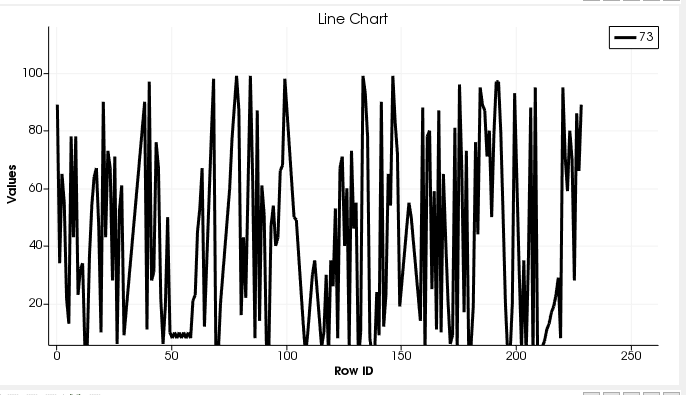
\includegraphics[scale=0.95]{Q1_L.PNG}
    \caption{Top: Histogram view, Bottom: Line Chart}
    \label{fig:q1}
\end{figure}
\clearpage
\textit{\\ Q.1:} Which number occurred the most frequently and how many times did it occur? \\ \\
\textit{Ans:} From the histogram of the data, we conclude that the number '10' occurred the most times - it occurred 10 times. 

\textit{\\ Q.2:} How many numbers were never used by the class?\\ \\
\textit{Ans:} Again from the histogram and line chart views, it can be concluded that 14 numbers (between 0-99) were never used in this class of data. The respective numbers are: 33, 38, 39, 48, 57, 58, 69, 75, 82, 84, 85, 91, 92, and 94. 

\textit{\\ Q.3:} Line Charts: Follow the same method as for histograms to render the line chart. Please add the left title as “Value” and the bottom axis title as the “Row ID” through the properties panel. Also, change the line thickness to 3 units. \\ \\ 
\textit{Ans:} Please look at the diagrams of Fig. 1 on the previous page.
\clearpage

\subsection{Visualization of 2d Image}
\paragraph{Ans} The results from the workspace in ParaView are attached below. The ParaView state is attached in the submission. 
\begin{figure}[!h]
    \centering
    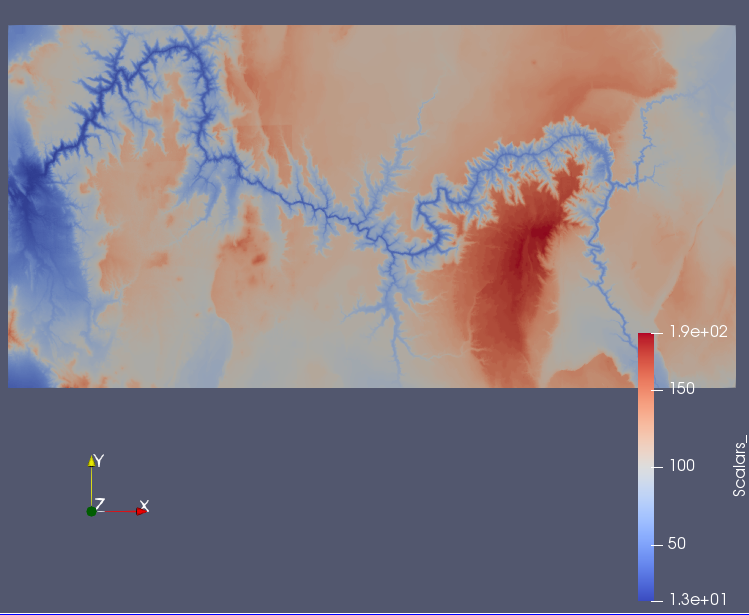
\includegraphics[scale = 0.50]{Q2_Orig.PNG}
    
    \vspace{1 cm}
    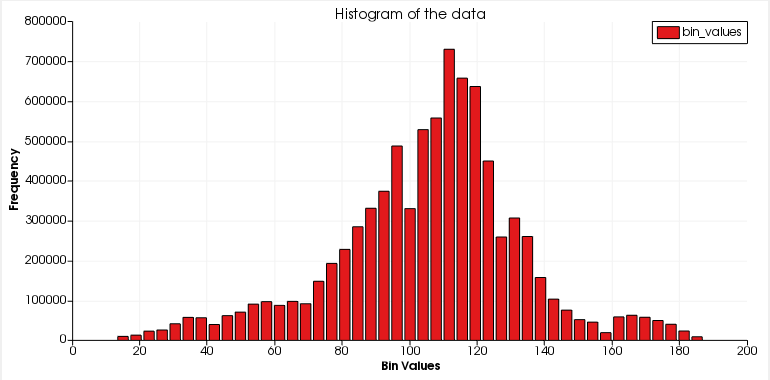
\includegraphics[scale = 0.50]{Q2_H.PNG}
    
    \vspace{1 cm}
    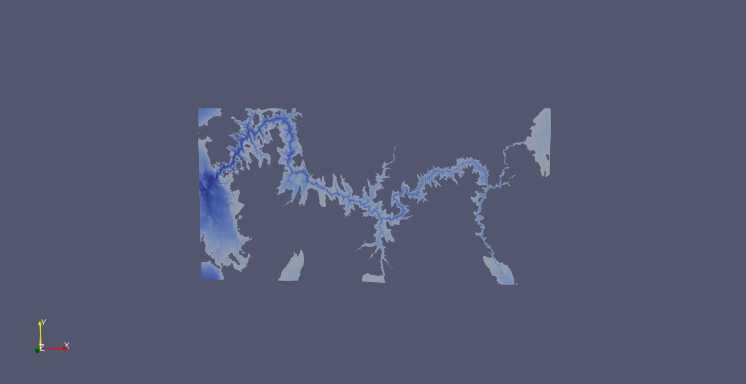
\includegraphics[scale = 0.50]{Q2_R.PNG}
    \caption{Top: Original data (w/o processing), Middle: Histogram view, Bottom: Riverbed (after Thresholding)}
    \label{fig:q2}
\end{figure}
\clearpage
\textit{\\ Q.1:} What threshold did you use for capturing the riverbed? Experiment with other thresholds and explain what features you may or may not have missed with this approach. \\ \\
\textit{Ans:} I used Histogram plot (bins = 45) as a head-start to understand what is the meaning of the intensity values for this data. After playing with different threshold values, I  finally settled on the threshold range with Minimum = 10 and Maximum = 90. I started the variations with minimum value as 0 but then I realized that although the river part is low intensity in this data there are other parts like shore of a river which are low intensity. So, instead of starting at 0, I started at 10 so as to capture only the river parts. Similarly, I tried maximum value variations above 80 and found the best result on 90. After this point, I was getting ground (brown) area also. I also tried different orientations and slicing etc. to understand the data. 

\textit{\\ Q.2:} Using the Information panel, report the number of points in the thresholded image. Note that ParaView automatically creates cells from an input image, implicitly forming a structured quad mesh. \\ \\
\textit{Ans:} From the information tab in the thresholded image, the data found is as follows:

Number of points = 2053863
Number of cells = 2010557

\clearpage

\subsection{Exploring Data on Polygonal Meshes}
\paragraph{Ans.} The state file associated with this question can be found in zip. For this question, I managed to get the required blue cylinder using the clipping planes as well as the thresholding approach. As far as the process goes, I first clipped the structure into half and then created a histogram to see the different intensity values and try to understand them. I found that essentially the 'blue' color is the one which is in the lowest intensity and with lowest occurrences. Then, I added a threshold filter and set up the min and max values as 0 and 40 (there was a white piece in the cylinder). Finally, to count the number of ventilation slots, I eased up the process a bit by just considering half of the cylinder because it's a symmetric figure. I counted the slots there and then doubled it to calculate it for the whole cylinder. The results are as follows:

\begin{figure}[!h]
    \centering
    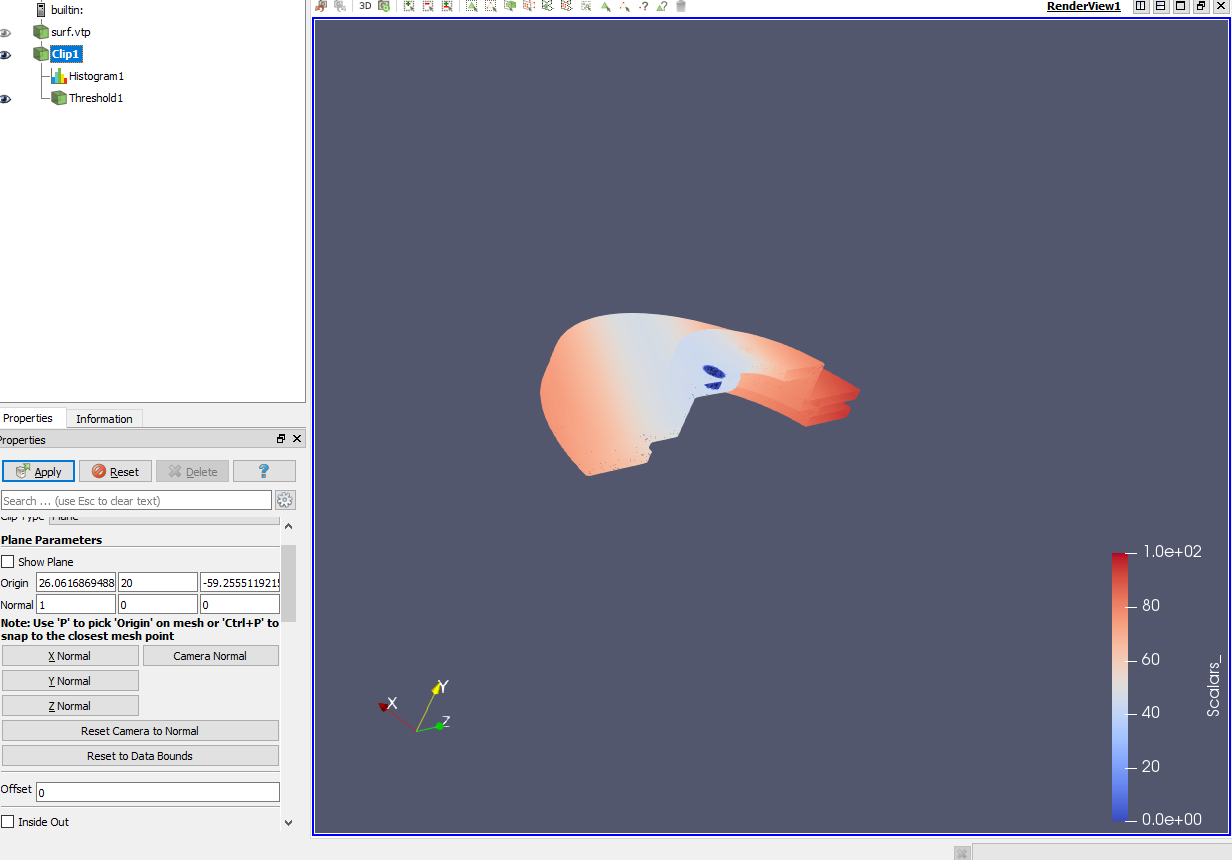
\includegraphics[scale = 0.45]{Q3_Clip.PNG}
    
    \vspace{1 cm}
    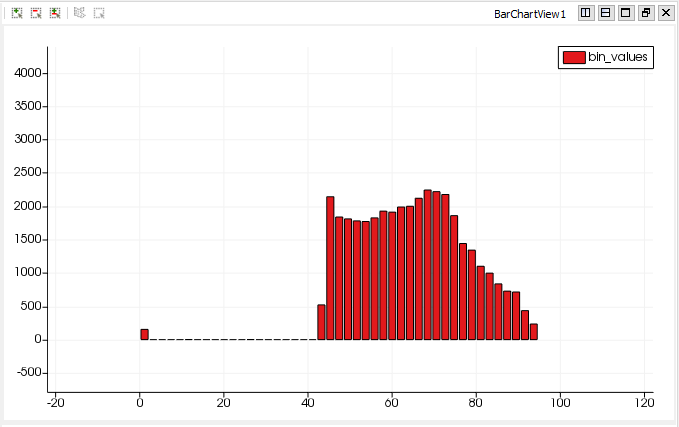
\includegraphics[scale = 0.55]{Q3_H.PNG}
     \caption{Top: First Half Clip, Bottom: Histogram after Halving}
    \label{fig:q31}
\end{figure}

\begin{figure}[!h]
    \centering
    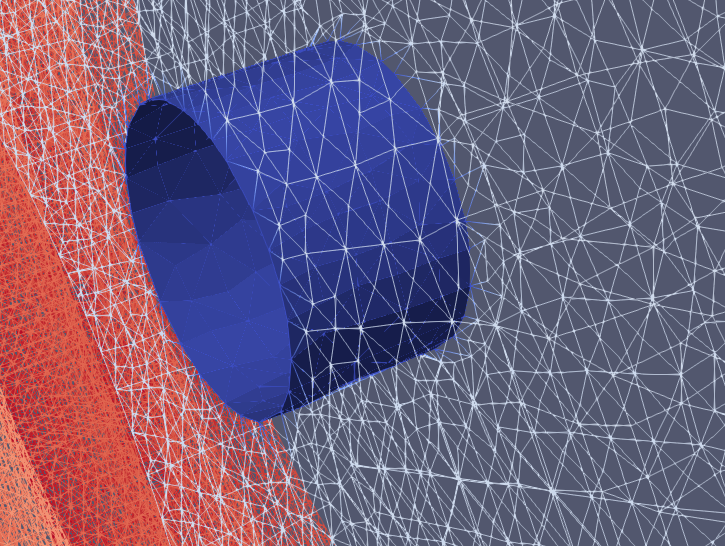
\includegraphics[scale = 0.60]{Q3_Threshold(0-5).PNG}
    
    \vspace{1 cm}
    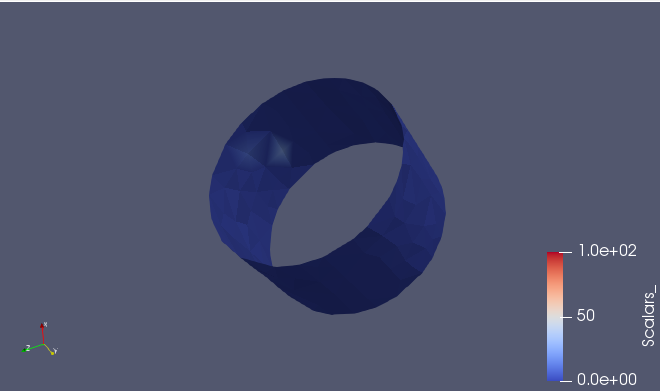
\includegraphics[scale = 0.60]{Q3_T(0,40).PNG}
    
    \caption{Top: Image after thresholding on the original wire-frame, Bottom: Thresholded Image obtained from clipped figure}
    \label{fig:q32}
\end{figure}

\begin{figure}[!h]
    \centering
    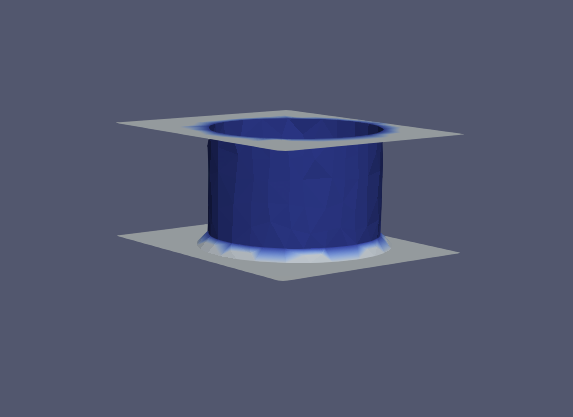
\includegraphics{Q3_Final_Clip.PNG}
    
    \vspace{1 cm}
    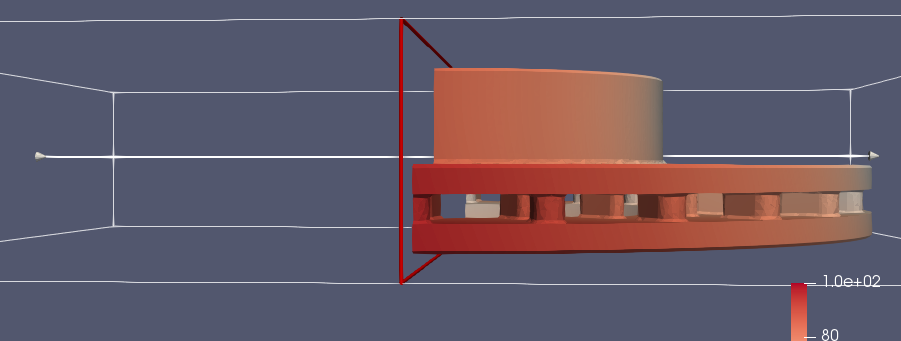
\includegraphics[scale = 0.70]{Q3_Ventilation.PNG}
    
    \caption{Top: Final Clipped image of the blue cylinder by using several clipping planes, Bottom: Half Clipped version of cylinder to count the ventilation slots (utilizing symmetry)}
    \label{fig:q32}
\end{figure}
\clearpage

\textit{\\ Q.1:} What were the minimum and maximum values that best captured the single cylinder associated with the bolt’s cylinder? \\ \\ 
\textit{Ans:} The final threshold value range I used to get the blue cylinder out is Minimum = 0 and Maximum = 40. \\ Ideally, it should be only 0 but we know that no data is perfect, and all datas have some noise associated in it. In our case, this can be seen in form of a few white spots on the cylinder (Fig. 4). To construct the whole cylinder without any gaps left out, we had to chose our max. threshold value as 40 so as to capture the noisy white part as well.  

\textit{\\ Q.2:} How many ventilation slots are there?  \\ \\ 
\textit{Ans:} Ventilation Slots in Half clipped figure (Fig. 5b) = 12 \\
Total number of ventilation slots = 12*2 = 24

\textit{I am considering one air hole between two pillars as one slot.}

\clearpage
\subsection{Visualization of 3D Images}
\paragraph{Ans. } I used multiple slicing planes here to get the required results. Then, the images can be arranged in a 2D plane by using the in-built options. The results are attached as follows:
\begin{figure}[!h]
    \centering
    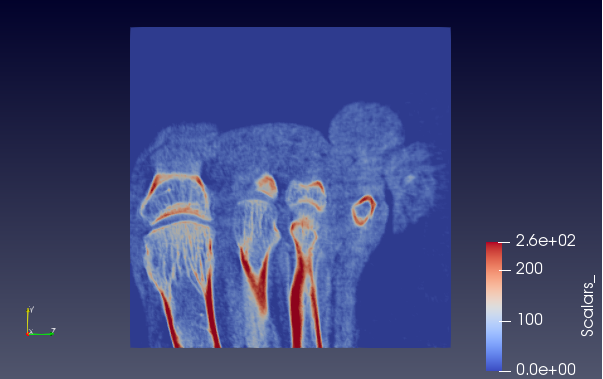
\includegraphics[scale = 0.6]{Q4_X.PNG}
    
    \vspace{1 cm}
    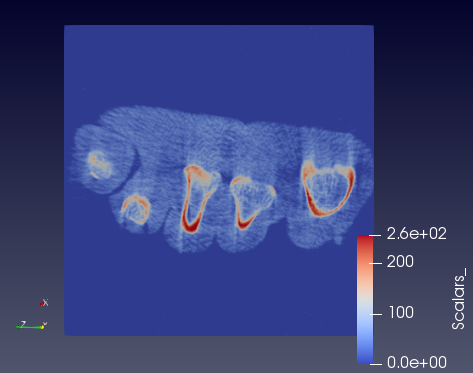
\includegraphics[scale = 0.7]{Q4_Y.PNG}
    
    \vspace{1 cm}
    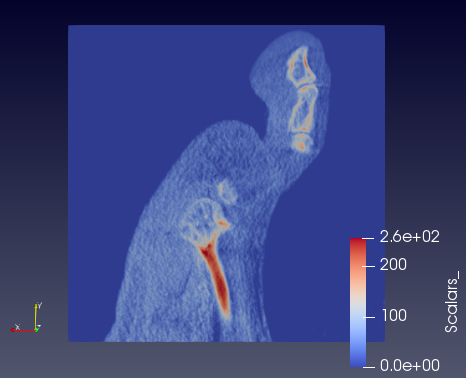
\includegraphics[scale = 0.7]{Q4_Z.PNG}
    \caption{Top: X-Normal Slice, Middle: Y-Normal Slice, Bottom: Z-Normal Slice}
    \label{fig:q32}
\end{figure}

\begin{figure}[!h]
    \centering
    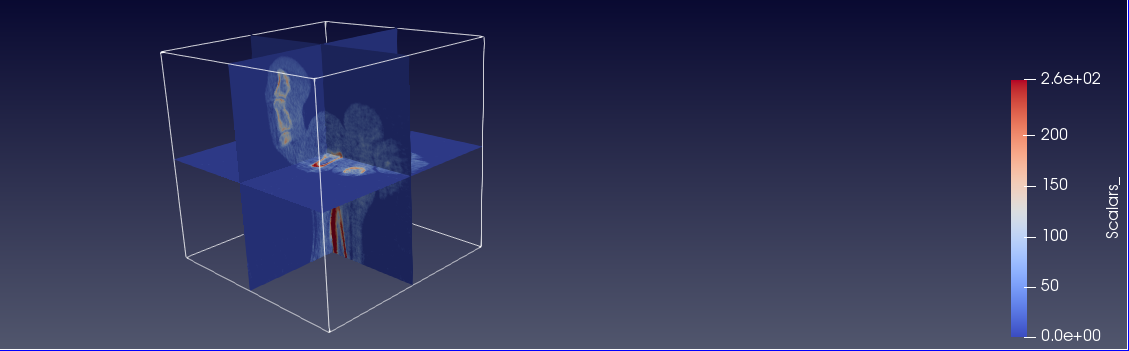
\includegraphics[scale = 0.6]{Q4_XYZ.PNG}
    
    \vspace{1 cm}
    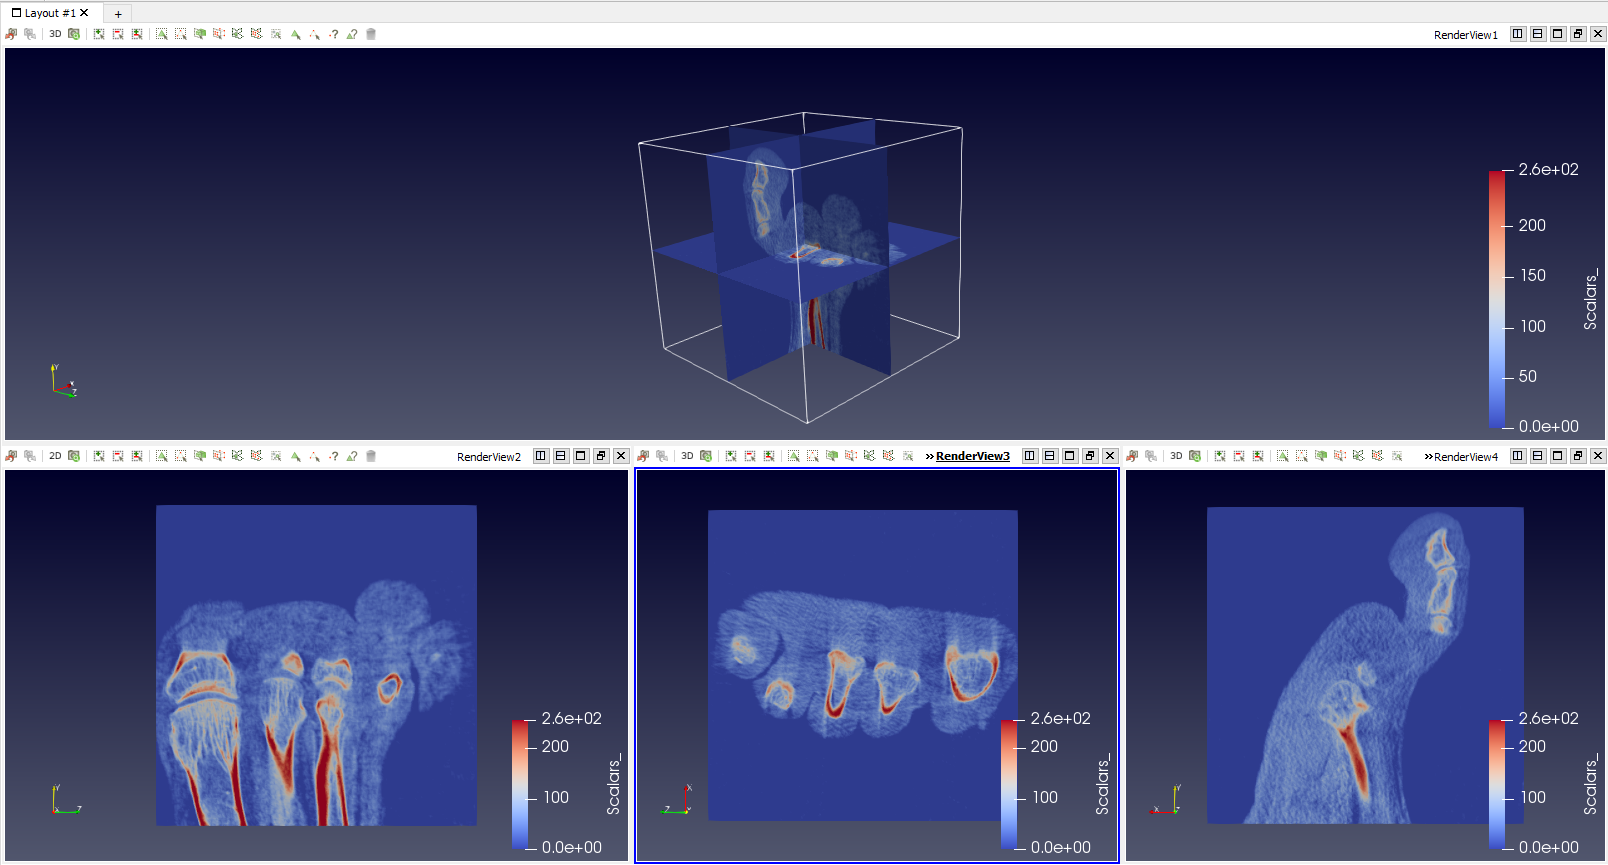
\includegraphics[scale = 0.42]{Q4.PNG}
    
    \caption{Top: X-Normal, Y-Normal, Z-Normal Slice rendering in one Outline, Bottom: Compiled Results}
    \label{fig:q32}
\end{figure}

\clearpage

\section{Part 2 - Code with Python Script}
\subsection{Use batch script to create a pipeline}
\paragraph{Ans.} The python script to run the program is attached with the solutions. Please refer Readme file for detailed instructions on running it. I have simply used the for loop to replicate the structure of an arrow in both the questions. I also set the tip resolution parameter to 12 for both the parts of this question. The results are as follows:
\begin{figure}[!h]
    \centering
    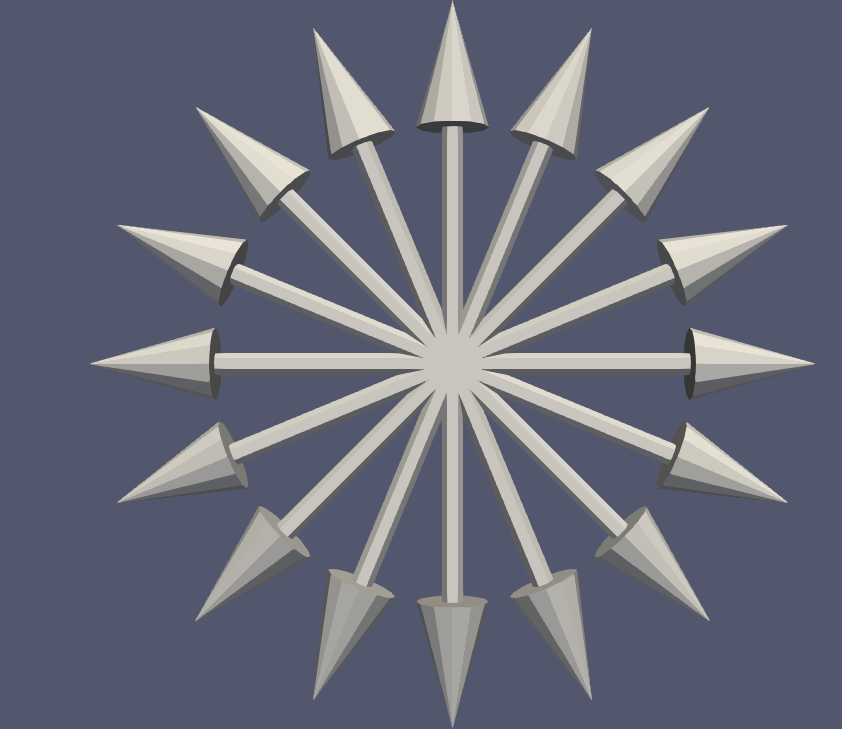
\includegraphics[scale = 0.4]{Q5_1.PNG}
    
    \vspace{1 cm}
    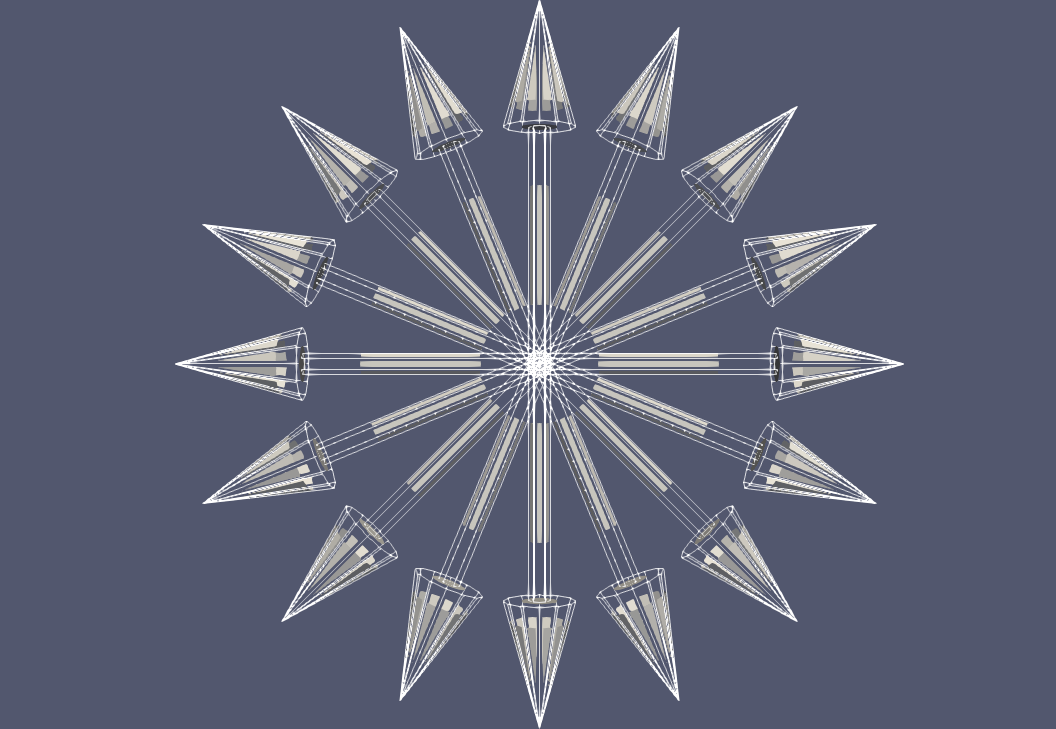
\includegraphics[scale = 0.33]{Q5_2.PNG}
    
    \caption{Top: 16 Arrows at Equal Distance, Bottom: 16 Arrows (with Shrinks and Extracted Edges) at equal distance}
    \label{fig:q32}
\end{figure}

\clearpage

\subsection{Read file and process it with Python script}
\paragraph{Ans.} The python script to run the program is attached with the solutions. Please refer Readme file for detailed instructions on running it. Here, I learned about a lot of commands like PlotOverline, Splitting Layouts etc. from the trace files that I got after doing all the operations in the ParaView. For conversion of this 2D image to a 3D map, I am using Warp Filter on the dataset. After playing with the scale factor, I found that the scale factor of 1.25 is the best one to visualize the dataset in 3D form. Here, we are just dealing with scalar values so all the filters, plots etc. are presented for the scalar values. The results are as follows: \\ \\ 
\begin{figure}[!h]
    \centering
    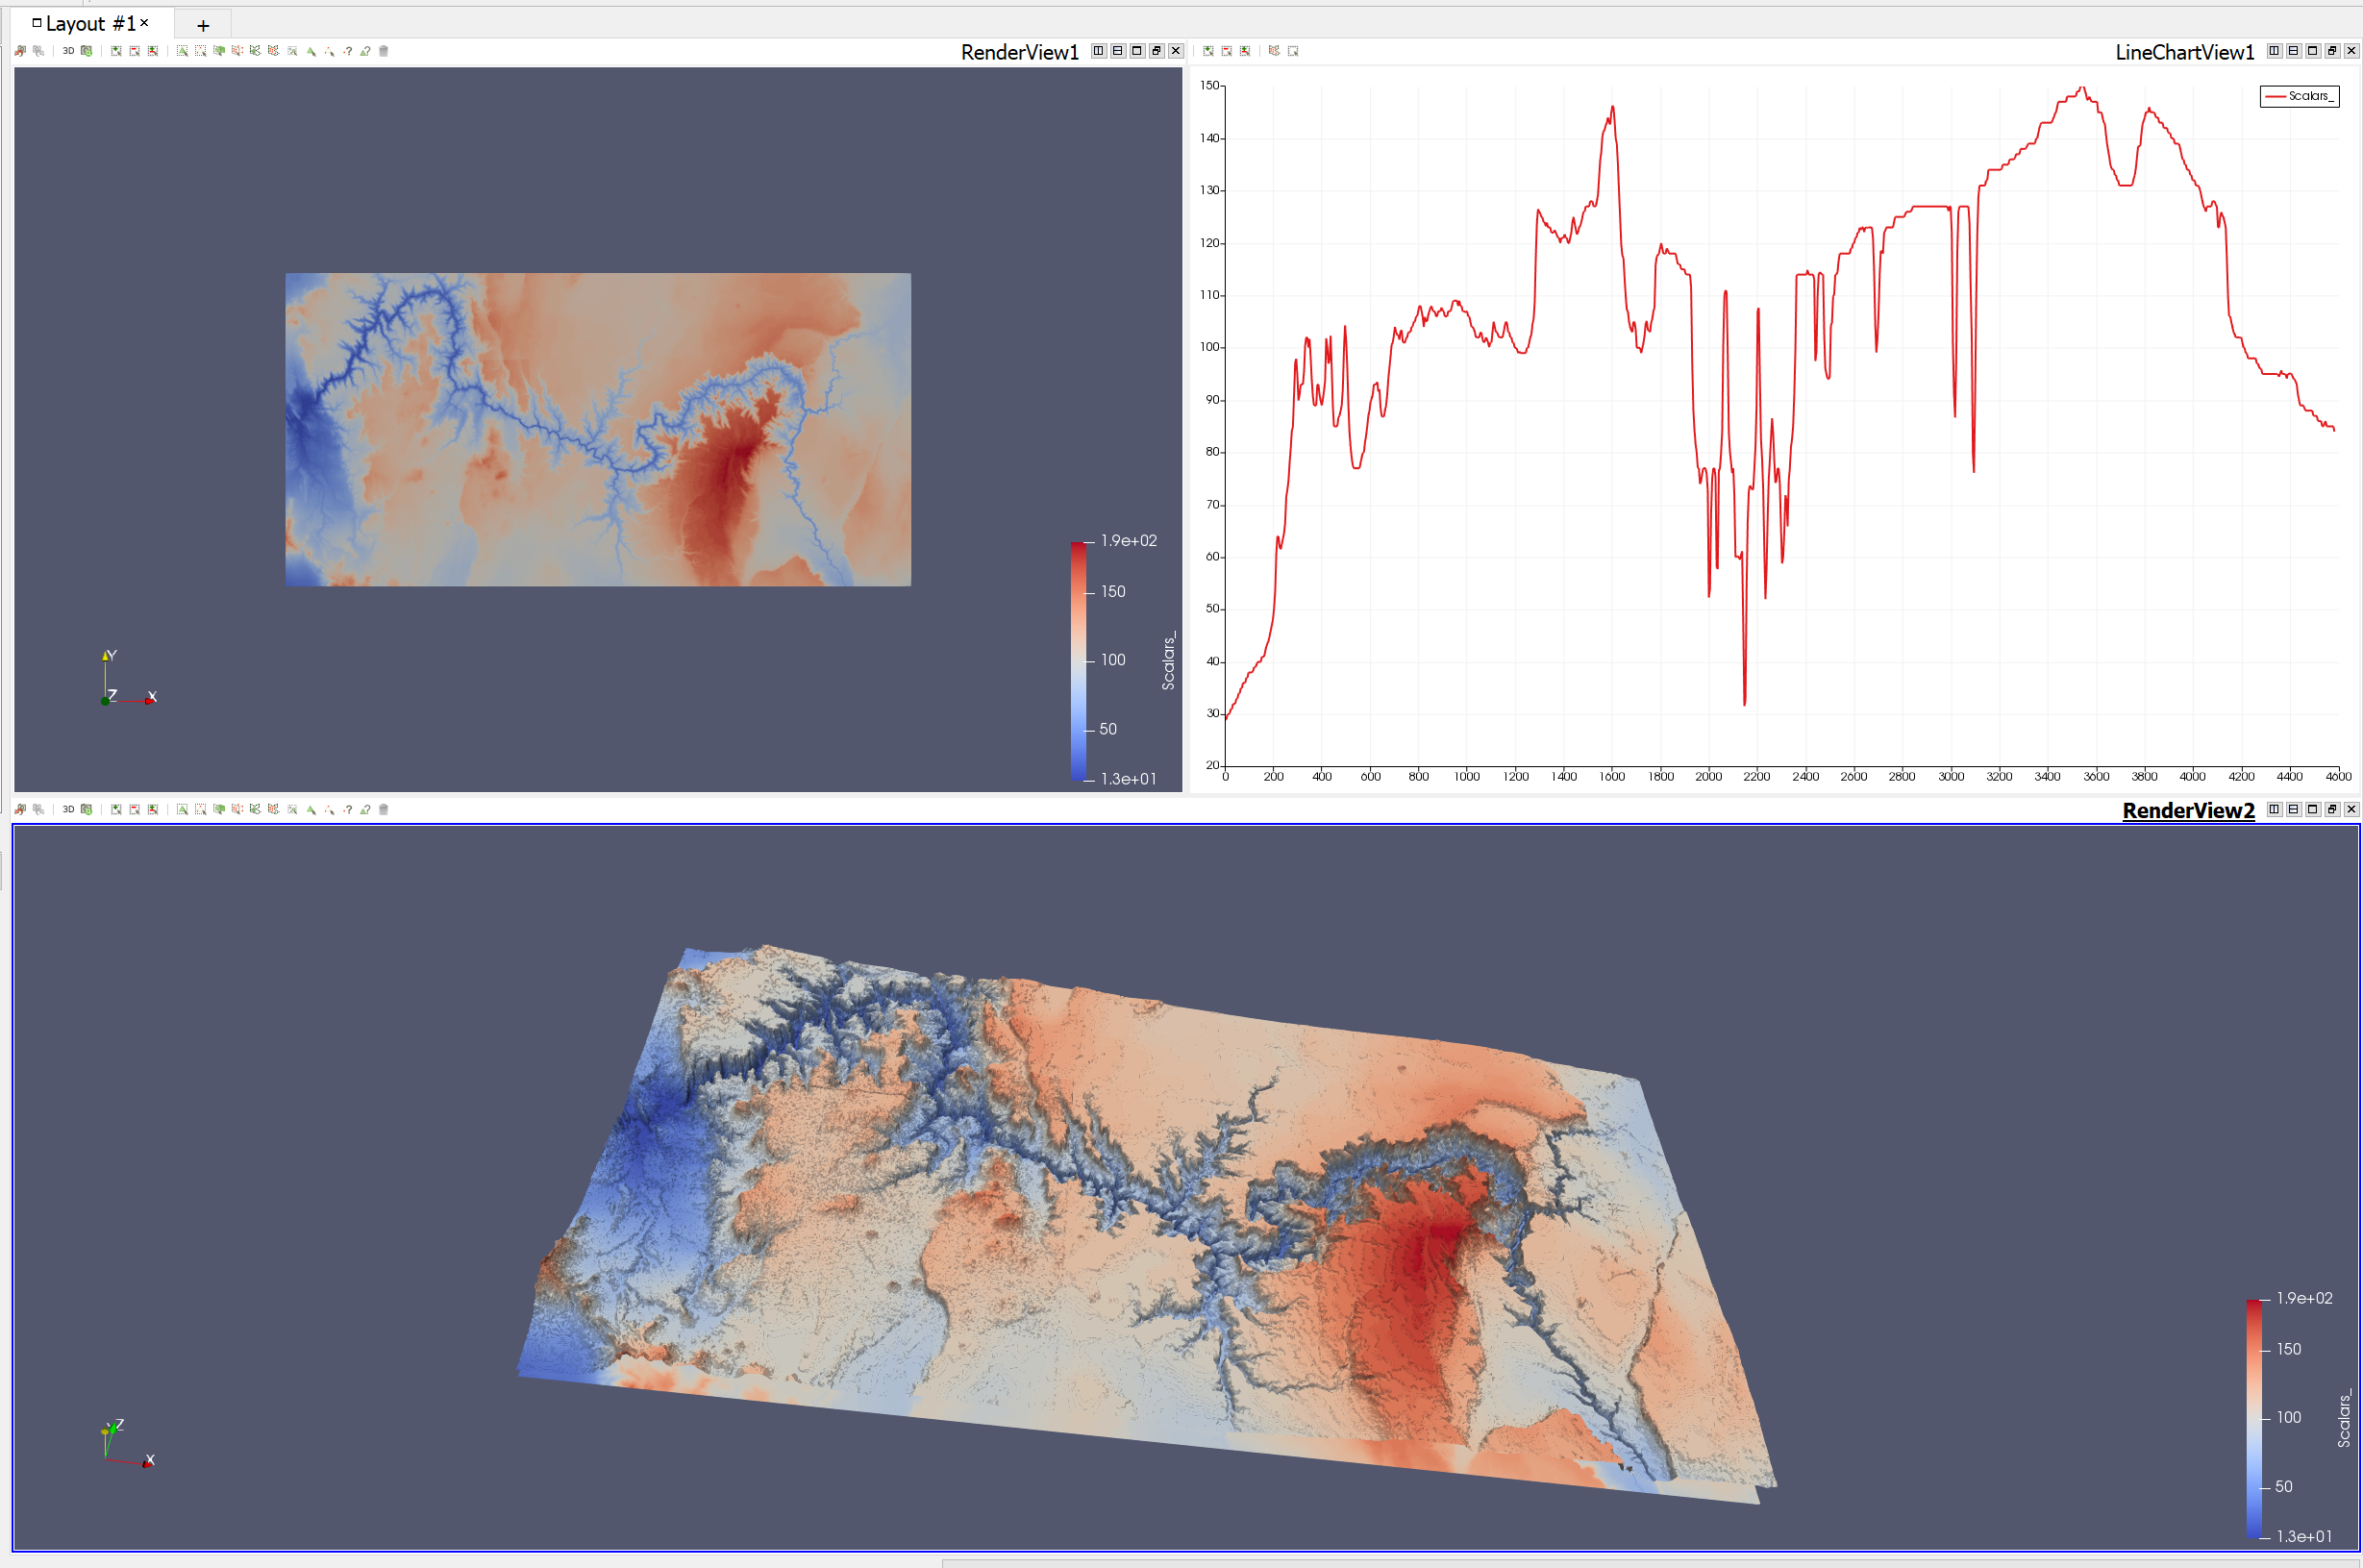
\includegraphics[scale = 0.53]{Q6.PNG}
    \caption{Top left: Original 2D View of Dataset, Top Right: Overline Plot for the Data, Bottom: 3D Map generated by applying Warp Filter on the Dataset }
\end{figure}
\clearpage
\section{References}
\begin{enumerate}
    \item ParaView Tutorials and Handbook
    \item Python Tutorials
\end{enumerate}
\end{document}